\documentclass[authoryear,1p,12pt]{elsarticle}
\usepackage{amsmath}
\usepackage{amssymb}
\usepackage[mathlines,displaymath]{lineno}
\usepackage{graphicx}
\usepackage[all,2cell,dvips]{xy}
\usepackage{natbib}
\usepackage[usenames,rgb]{xcolor}
\usepackage{ucs}
\usepackage[utf8]{inputenc}
\usepackage{array}
\usepackage{longtable}
\usepackage{calc}
\usepackage{multirow}
\usepackage{hhline}
\usepackage{ifthen}
% \usepackage{babel}
\usepackage{tcolorbox}
\newtcolorbox{mybox}{colback=grey!5!white,colframe=red!75!black}
\usepackage{setspace}
\usepackage{verbatim}
\usepackage{etaremune}
\usepackage{url}
% \usepackage{color}
\usepackage{graphicx}
\usepackage{natbib}
% \usepackage[latin1]{inputenc}
\usepackage{array}
\usepackage{float}
\usepackage{wrapfig}
\usepackage{hyperref}
%\floatstyle{boxed}
%\restylefloat{figure}

\newcommand{\etal}{{et~al.{}}}
\newcommand{\ie}{{i.~e.{}}}
\newcommand{\eg}{{e.~g.{}}}
\newcommand{\viz}{{viz.{}}}
\newcommand{\etc}{{etc.{}}}
\newcommand{\apriori}{{a priori{}}}
\newcommand{\vv}{{vice versa{}}}
\newcommand{\cf}{cf.{}}
\setcounter{tocdepth}{3}
\usepackage{tikz}
% \newcommand{\carlos}[1]{\textcolor{Red}{#1}}

% Text layout
\topmargin 0.0cm
\oddsidemargin 0.25cm
\evensidemargin 0.25cm
\textwidth 15.5cm
\textheight 21cm

\vspace{0.1 in}
\pagestyle{myheadings}
\markboth{CJ Meli\'an \& VM Egu\'iluz}{CJ Meli\'an \& VM Egu\'iluz}


\begin{document}
\section{{\bf Title: Deep process-based learning networks in biological, technological and economical systems}}
%Alternative title: Deep process-based learning networks platform 

\section{{\bf Summary}}
%2,000 characters: most relevant aspects; goals; duration in months}
We are in a enthralling scientific era. We have the computer power,
the open-source tools, the know-how in many specialized fields and the
team capabilities to infer complex patterns from highly heterogeneous
data. We are in a period where novel analytical methods and data are
being fussioned at an incredible speed. Yet, deciphering the strength
of process-based feedbacks underlying patterns of big multilayer data
across fields is at a very incipient stage (Figure 1). Our proposal
aims to fussion data with process-based feedbacks to disentangle the
mechanisms underlying complex empirical patterns. First, we will
develop an open-source automated research platform accounting for data
integration, complexity reduction, inference, validation,
visualization and reporting generation (Figure 2). Second, we will
test the platform to decipher the strength of the feedbacks underlying
Earth Biodiversity patterns accounting for multilayer network data
(Figures 3 and 4). Our research goals contain two main milestones for
a 24 months duration plan (Figure 5): The first milestone will be the
deployment of an automated research platform by the end of the first
year. The second will test the automated research prototype with Earth
biodiversity data as a case study to be developed during the second
year to show mechanistic feedbacks inference in complex empirical
patterns.

\newpage

\section{Background and objectives}

% degree of innovation technical, economic and social importance
Specialization has produced an immense gain in detailed knowledge at
each of the levels and scales studied across many scientific
disciplines. However, integrating the information obtained in
specialized fields with existing technologies and methods in natural,
technological, social and economical systems still present many
challenges. Despite rapid advances of automated research platforms
facilitating data integration accounting for parts of the research
cycle\footnote{This is by no means an exhaustive list but it gives an
  indication of the many projects taking currently place:
  \href{https://www.nterminal.com}{NakamotoT},\href{https://cloud.google.com/bigquery/}{BigQuery},\href{https://www.automaticstatistician.com/index/}{Automated
    statistician},\href{http://www.modulos.ai/}{Modulos},\href{https://ai.google/}{Google
    AI},\href{https://iris.ai}{Iris}\href{https://github.com/DS3Lab/easeml}{easeml}}
open-source automated research platforms are still at a very incipient
stage of development.

One of the reasons automated research platforms are still at a very
incipient stage of development is because most methods in data science
and other scientific disciplines have been considered classically as
distinct fields. This is rapidly changing due to the current
scientific ecosystem. We are at an stage where merging methods from
distinct fields is radically transforming the discipline boundaries,
the reproducibility of science and our predicting-understanding
power\citep{Reichsteietal2019}. Many recent approaches applying deep
learning methods in biology, economics, social and technological
systems have mostly focused on pattern detection within one level of
organization \citep{Sheehan&Song:2016}. While this might produce
additional gain in detailed knowledge at each level for understanding
such systems, it remains unknown how many layers are going to be
needed for maximizing predictive- and process-based knowledge in
biological, economical social and technological systems (Figure 1).

Gaining predictive and understanding power need the merging of
distinct databases into hybrid deep process-based learning methods
accounting for many layers and the topology of the interactions within
and between the
layers\citep{Schmidhuber:2015,Ghahramani:2015,Melianetal:2018,Reichsteietal2019}. Many
methods from data science and biological, economical and technological
systems share fundamental properties (i.e., network-like patterns,
multiple layers, spatiotemporal dynamics, interdependent hieraqrchies
and feedbacks with interacting learning entities within and between
the layers, etc), and the full potential of these shared properties
have not been sufficiently explored combining big data with deep
process-based multilayer networks in automated research platforms
(Figure 2). In this regard, science, engineering and technological
landscapes require the integration of many layers to facilitate
automation, reproducibility, cooperation, new science of science
methodologies, and public access to the full research cycle and
research findings. Yet, technologies facilitating compactly
open-access to the full research cycle accounting for multilayer data
is currently not in place. Our research proposal aims to deploy a
multilayer automated network accounting fully for the research cycle
to provide decentralized and real-time open-access data-rule-knowledge
to gain informed decisions to help solve complex ecological, social
and technological problems.

Data driven multilayer process-based methods can increase the pool of
deep learning models in data science to understand more broadly the
connection between predictive power (i.e., pattern detection), and
understanding power (i.e., process-based inference). While conceptual
frameworks unifying different layers in many research fields is well
established, there is currently a lack of deep process-based learning
models accounting for many layers in biological, social, technological
and economical systems. Here is where data science can benefit to
further developing approaches unifying data driven patterns and
process based theory. The interaction between prediction and
understanding power can also advance synthesis in data-science by
gaining broader insights from deep pattern- and process- based
learning models that can be applied to other many fields.

  \begin{center}
    \hspace{0.25 in}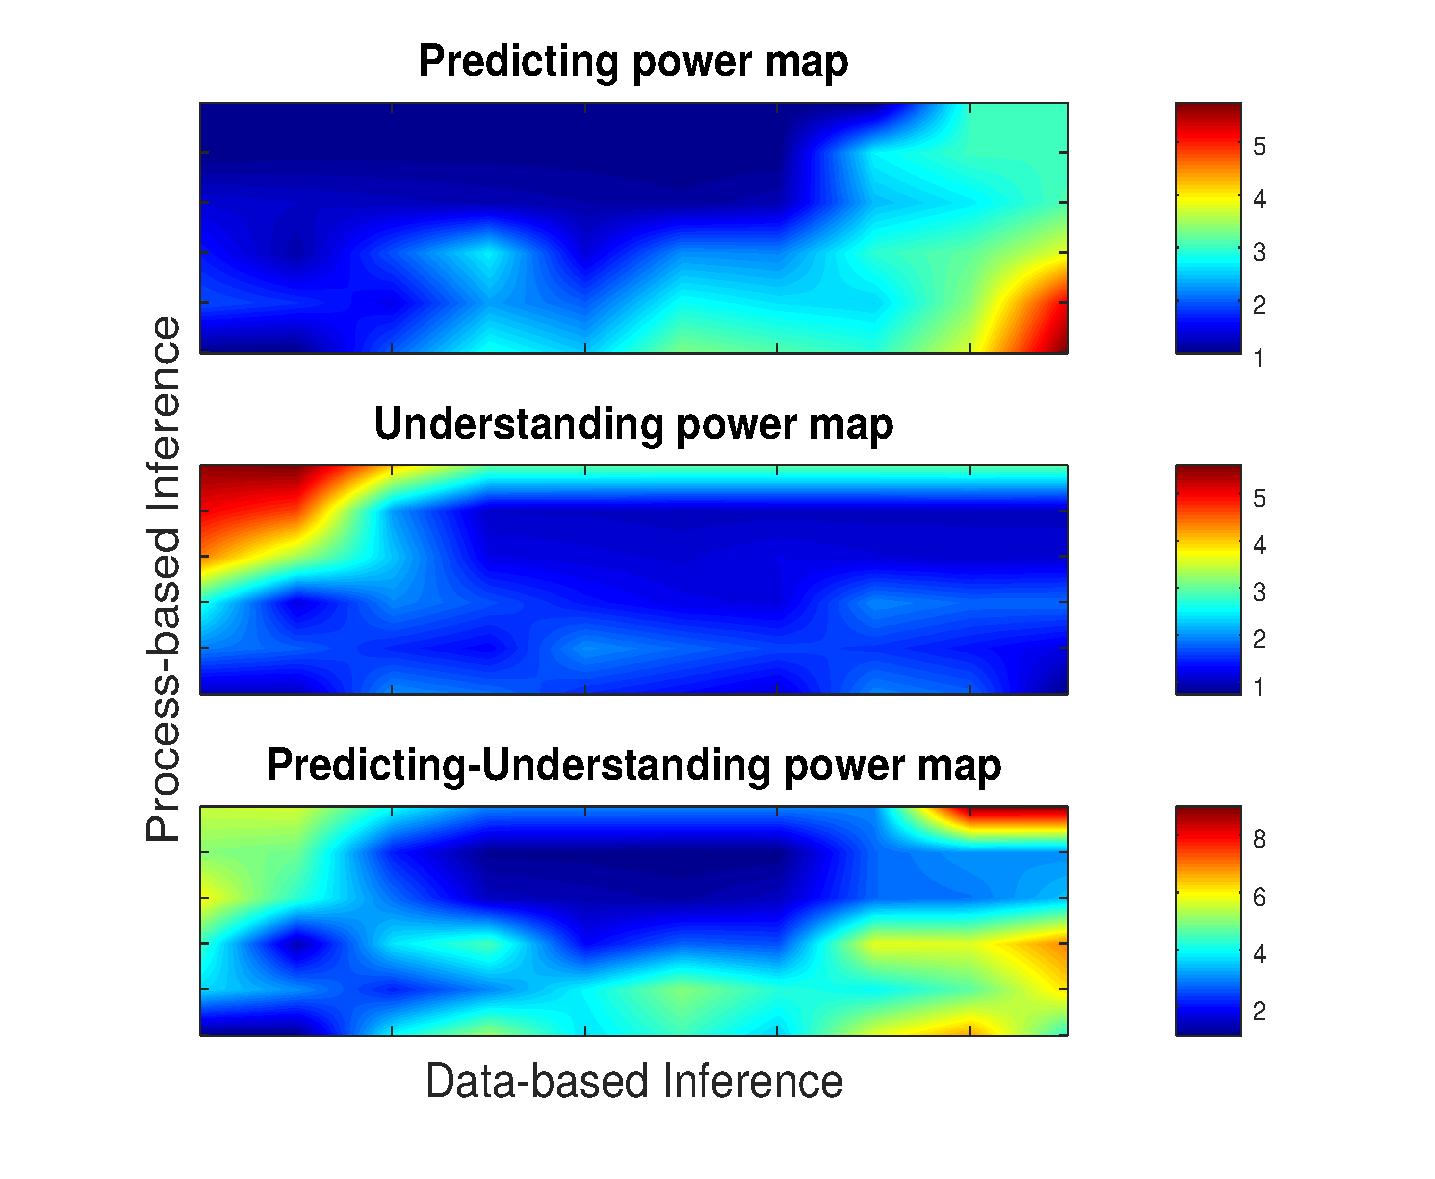
\includegraphics[width=0.85 \textwidth]{Figure3.eps}
     \end{center}
     \vspace{0.2 in}
     \caption{{\small {\bf Figure 1: Prediction power (top), understanding
         (middle), and prediction-understanding power maps
         (bottom)}. x-axis represents data-based inference (i.e.,
       gradient of AI methods from low (left) to high (right)
       predictive power). y-axis represents process-based inference
       (i.e., gradient of process-based methods from low (bottom left)
       to high (top left) understanding power). The gradient of
       predicting power map (top) shows a hot spot red area in the
       bottom right highlighting the region where AI methods best
       predict the empirical data. The gradient of understanding power
       map (middle) shows a red hot spot in the top left highlighting
       the region where the best mechanistic understanding occur. The
       predicting-understanding power map (bottom) shows the sum of
       the two previous maps highlighting a red hot spot where the
       best synthesis research joining predicting and understanding
       power of the empirical data might occur. The first research
       goal of this proposal aims to build an automated research
       platform to maximize the predicting and understanding power
       highlighted in the red hot spot of the predicting-understanding
       power map (bottom).}}

   \section{Research methodology}

   The project will introduce an automated research platform to
   facilitate open-access and neutral reports to gain informed
   decisions when solving complex social, environmental and
   technological problems. Current technologies for scientific inquiry
   are highly fragmented and thus only increase methodological
   robustness, reproducibility and the interactions with the public
   marginally. The first goal of this project is to propose a new
   hybrid-technology concept combining deep learning and automation to
   lay the foundation for a novel open-science ecosystem aiming to
   couple predictive and knowledge power in contemporary
   societies. Our first goal is not set out to deliver a finished
   automated research platform in the science ecosystem but to provide
   a science-enabled technology in establishing a prototype
   proof-of-principle for an open public-science ecosystem. Our second
   goal will test the platform with a Earth Biodiversity case study to
   show the possibilities of open automated reporting generation for
   the science ecosystem.

     \subsection{Goal 1: Automated data-driven platform}

     The science ecosystem requires multiple steps of information
     transfer among peers, the public, stakeholders and funding
     bodies. In this ecosystem, it will be key to have open and
     neutral access to full reports to gain informed decisions in
     complex societal, economical, environmental and technological
     problems. As a step towards neutral access to full reports and
     open science we aim to build an end-to-end research platform from
     data integration to reporting generation. The overall goal at
     this stage of the project is to deploy a protocol for
     implementing the algorithms for intra- and inter-layer automation
     of data integration, complexity reduction, inference, validation,
     visualization and reporting generation (Figure 2). We will deploy
     a diverse array of algorithms within each of the layers
     represented in the Figure 2. The following are the two key steps
     to build an automated research platform:

     \begin{itemize}
     \item Deployment of open-source packages for data integration,
       complexity reduction, inference and validation schemes (First
       top-three layers in Figure 2a). Despite open-source
       Extract-Transform-Load algorithms (ETLs) are rapidly evolving
       towards accounting for many aspects of data integration
       (formats, historical-real time, storage, dimensions, size,
       heterogeneity, multiple sources of bias, and spatiotemporal
       resolution), there is still a missing component in quantifying
       the robustness of knowledge that integrated data can provide
       throughout complexity reduction, inference, and validation. We
       will test the robustness of the open-source ETLs packages for
       merging datasets using simulated data (We will use empirical
       data during the second goal of the project, see section ``Work
       plan and calendar''). The top fourth layers in Figure 2b shows
       a first version of the algorithms and packages of the julia
       computing language to be integrated with the ETLs packages for
       data integration, complexity reduction, validation and
       inference.
     \item Deployment of knowledge graph algorithms
       \citep{Bonattietal:2018} to explore combinations of research
       paths in the multilayer network represented in Figure 2 (i.e.,
       sensu Renku open-source
       code\footnote{https://renku.readthedocs.io/en/latest/}). We
       will explore knowledge graphs in the multilayer network using a
       range of deep learning algorithms from bidirectional recurrent
       neural networks (BRNN) to feedforward neural networks (FNN) and
       reinforcement learning (RL) in both static and unknown and
       dynamic optimum\citep{Schmidhuber:2015}. This exploration will
       facilitate us to explore many properties of the automated
       platform like the robustness, reproducibility and bias of the
       knowledge-based algorithms to gain rule-based knowledge of the
       simulated data.
     \end{itemize}
     
     %SUMMARIZE MORE COMPACTLY THIS PARAGRAPH     
     %\cite{Webb2018,Heaven2019} The recent success of Artifical
     %Intelligence can be easily illustrated with applications to many
     %discipline. Examples could include machine learning nowcasts
     %lightening occurrence \cite{Mostajabi2019}, ...  astounding
     %performance in beating board and video games
     %\cite{Mnih2015,Silver2016}, computer vision that enables
     %self-driving cars \cite{Poggio2004,Krizhevsky2012}, medical
     %diagnosing \cite{Ferrucci2013}, ...

    
   %\begin{wrapfigure}{l}{0.86\textwidth}
  \begin{center}
        \hspace{-0.75 in}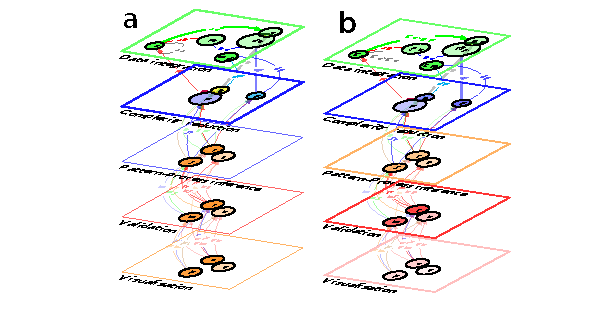
\includegraphics[width=1.1 \textwidth]{Figure4}
     \end{center}
     \vspace{-0.15 in}
     \caption{{\small {\bf Figure 2: Automated data-driven research
           platform:} {\bf a)} Automated data-driven prototype
         containing initially five layers: Data Integration,
         Complexity reduction, Pattern-process inference, Validation,
         and Visualization (Reporting generation not shown). Nodes and
         links represent algorithms and connections between two
         algorithms, respectively. The inter-layer interactions will
         be implemented using the open-Renku-Swiss Data Science Center
         platform\footnote{\href{https://renku.readthedocs.io/en/latest/}{Renku}}. The
         intra-layer interactions will be developed initially in julia
         language (other languages will come into play during the
         development of each layer). {\bf b)} A julia computing
         language prototype of an automated research platform. Nodes
         and links in each layer represent julia packages and
         interactions between two packages, respectively. The figure
         shows the julia packages for the Data integration layer
         containing the packages "Retriever.jl" ({\bf Re}), "Query.jl"
         ({\bf Qu}), "MySQL.jl" ({\bf My}), "SQlite.jl" ({\bf lite}),
         and "DataFrames.jl" ({\bf df}).}}
%\end{wrapfigure}

     \subsection{Goal 2: Deep-process based learning networks in Earth Biodiversity}
     
     We are in a massive human-driven biodiversity extinction with
     large uncertain consequences for Earth climate, life conditions
     and the stability of Earth (Figure 3). To gain predictive and
     understanding power in Earth Biodiversity research we are going
     to need to merge distinct databses into hybrid deep process-based
     learning methods accounting for many layers and the topology of
     the interactions within and between the
     layers\citep{Melianetal:2018}. Social, economical, technological
     and biological systems share fundamental properties (i.e.,
     network-like patterns, multiple layers, etc) and they might
     contain interdependent hierarchies and feedbacks with interacting
     learning entities within and between the layers (Figure 4). Yet,
     the full potential of these shared properties have not been
     sufficiently explored in the context of open automated research
     platforms. Our second goal will integrate different biological
     layers into the platform developed during the first step of this
     proposal to explore contrasting scenarios of Biodiversity
     dynamics accounting for feedbacks within and between layers
     (Figures 3 and 4 and section below) (See below the section
     ``Modeling deep process-based learning networks for Earth
     Biodiversity'').

 \begin{center}
       \includegraphics[width=0.65\textwidth]{Figure1}
  \end{center}
     %\vspace{-0.7 in}
  \caption{{\bf Figure 3: Biodiversity is declining globally at
      unprecedented rates}. Map showing the remaining populations of
    native species across many taxa as a percentage of their original
    populations. Blue areas are within proposed safe limits, and red
    areas are beyond these limits. For furhter information please
    check the original work at
    {http://www.nhm.ac.uk/discover/news/2016/july/biodiversity-breaching-safe-limits-worldwide.html}.}
     
\subsubsection{Modeling deep process-based learning networks for Earth Biodiversity}

We will infer process-based species distribution maps accounting for
different biological layers and deep learning networks (See Goal
1). Most datasets in biodiversity are collections of small data. In
areas such as species ranges and species interactions, there is a
large amount of data, but only a relatively small amount of data match
the species ranges or the species interactions with lower biological
level data as the gene architecture or the phenotypes. To account for
such uncertainty we will use a formalism considering the heterogeneity
at individual level\citep{Ghahramani:2015} coupling the
gene-to-phenotype map to populations, and interactions among
phenotypes to communities and species ranges, so that information can
be borrowed from other similar levels across the landscape. We will
develop the formalism into hierarchical Bayesian neural networks to
generate biodiversity distribution maps accounting for biotic, abiotic
and migration traits that can be compared against the empirical
distribution patterns. We will consider many populations characterized
each by individuals containing $\mathrm{T}$ normally distributed
traits (i.e., biotic, abiotic, and migration traits represented as
{\bf $z_{i}$} with $i$ the biotic, abiotic or the migration
trait). Populations will be located in a network of
discrete/continuous sites guided by long/lat empirical data connected
by migration events and the local population demography will be driven
by the temporal dependent fitness function accounting for trait
architecture following
\begin{equation}
  \hspace{-0.05 in} \mathrm{W({\bf z_{i}})}^{t}_{jx} = exp[\left -\gamma(((\mathrm{\bf z_{i}}^{t}_{jx} - \mathrm{\bf \theta}_{jx})^2)^T \mathrm{\bf \omega}^{-1} (\mathrm{\bf z_{i}}^{t}_{jx} - {\bf \mathrm{\bf \theta}_{jx})^2)\right],\hspace{-0.15 in}
\end{equation}
where $\mathrm{\bf (z_{i})}^{t}_{jx}$ is the vector of trait values of
phenotype $z$ at time $t$ for species $j$ and site $x$,
${\bf \theta}_{jx}$ is the multivariate fitness optimum of species $j$
in site $x$, ${\bf \omega}$ is the covariance matrix\citep{Lande:1980,
  Melo&Marroig:2014}, and $\gamma$ determines the interaction
sensitivity to deviations from the biotic, abiotic and migration
optimum. If the covariance matrix, ${\bf \omega}$, is diagonal, then
we are in a no correlated stabilizing selection scenario. Each trait
is independently evolving and the connections within and between each
biological level are modular and mostly weak. Adding covariation among
traits will result in correlated stabilizing selection with strong
interactions within and between each biological level. The population
dynamics of species $j$ in site $x$ is then given by
{\begin{equation}{\frac {dN_{jx}}{dt}}&= r_{jx}(F(W({\bf z})) +
    m_{jx}(F(W({\bf z})),\end{equation}} where $r_{jx}$ and $m_{jx}$
are the multivariate fitness-dependent intrinsic growth and migration
rate, respectively. The first scenario accounting for independently
evolving traits will be our proxy for quasi-independent levels
considering modularity within- and between-layers (i.e., a highly
modular pleiotropy matrix determining the genotype-phenotype map and a
highly modular within- and between-species interactions with most
interactions weak or zero across the landscape). Such scenario will
produce a non- or weakly-interactive species biodiversity map. The
second scenario will account for correlated traits and we will
consider this scenario as our proxy for feedbacks within and among
layers. We will explore a range of topologies from bidirectional
recurrent neural networks (BRNN) to feedforward neural networks (FNN)
and reinforcement learning (RL) in both static and unknown and dynamic
optimum\citep{Schmidhuber:2015}. This scenario will produce an
strongly-interactive species biodiversity map. We will disturb both
scenarios following random and non-random disturbance regimes (i.e.,
removing specific interactions, abundances and habitats) and will
quantify responses to disturbances using a variety of metrics, from
local, regional and global biodiversity
metrics\citep{Melianetal:2018}.

    \begin{center}
  \vspace{-0.5 in}
        \hspace{-1.25 in}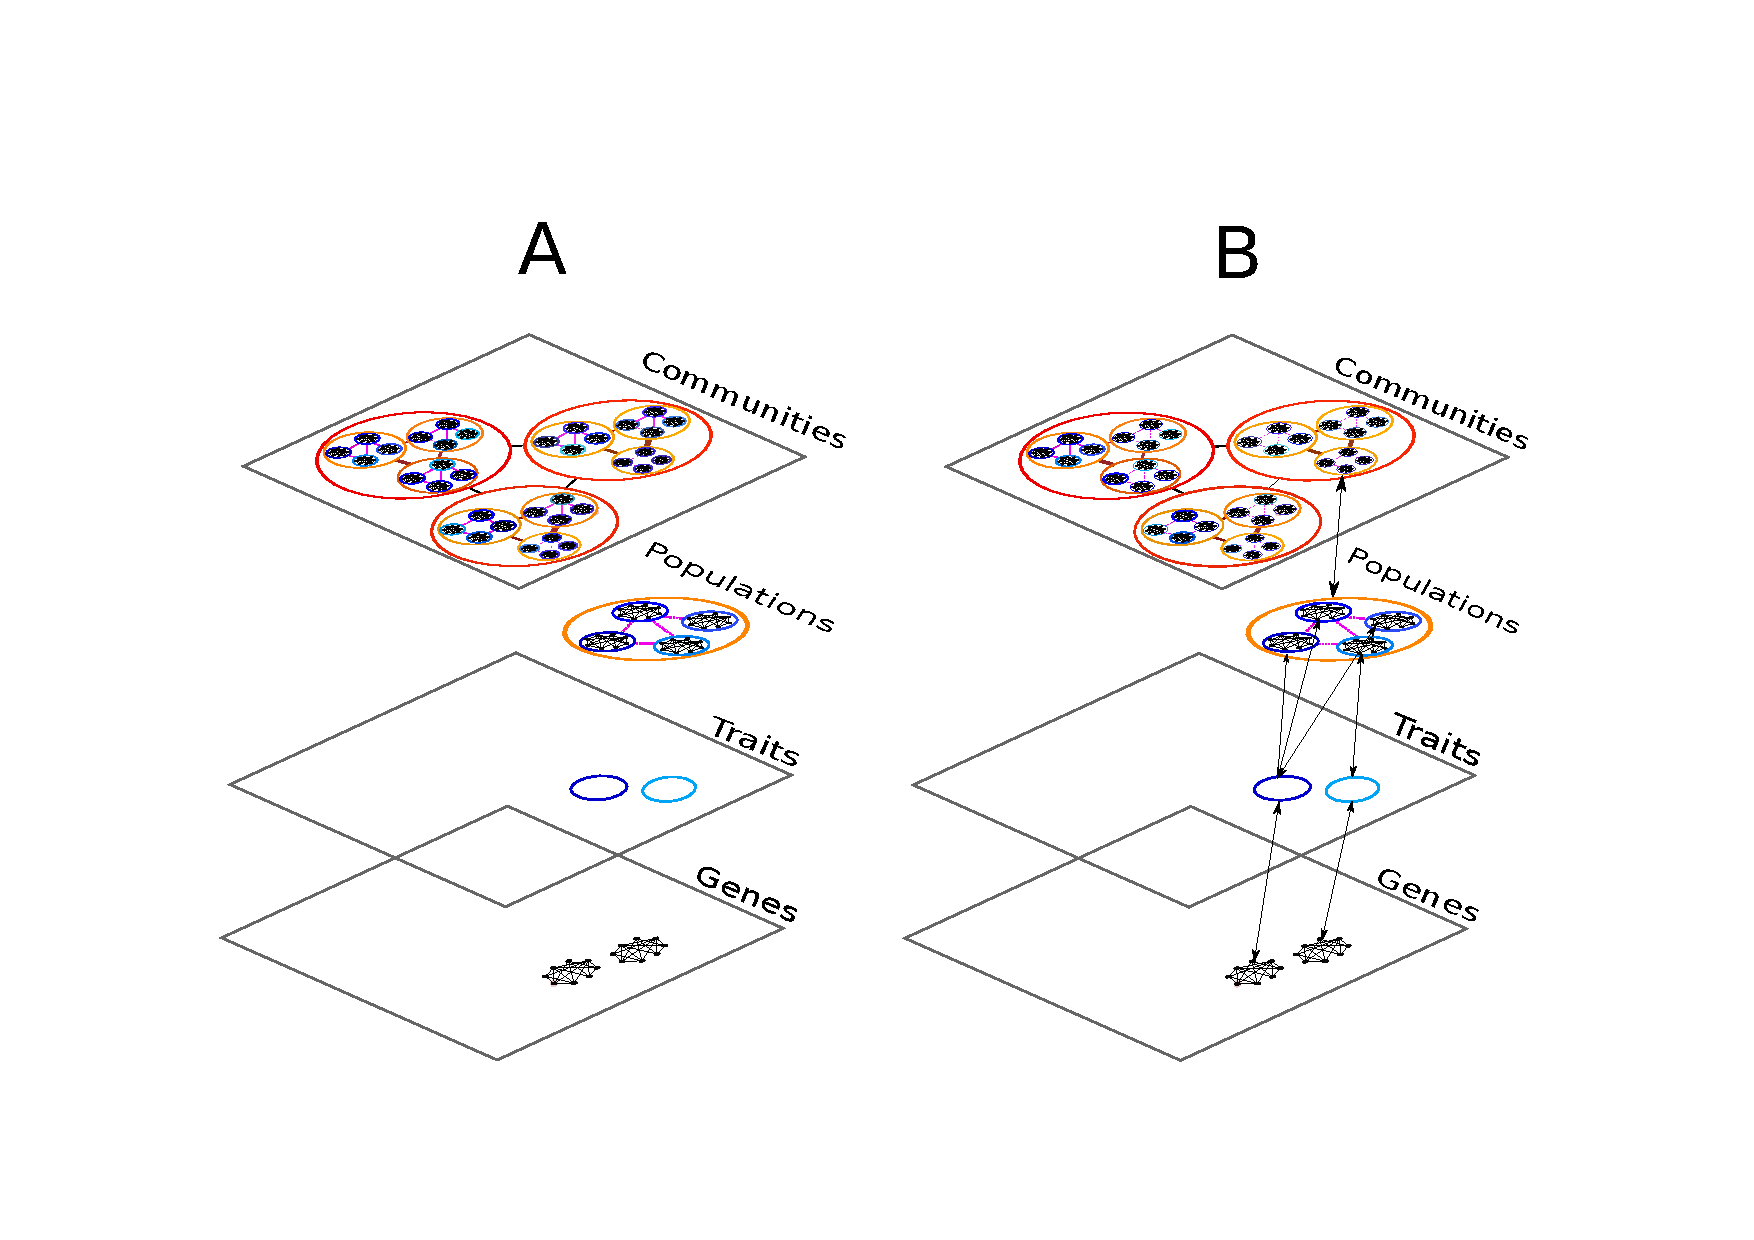
\includegraphics[width=1.2\textwidth]{Figure2.pdf}
\end{center}
     %\vspace{-0.5 in}

\caption{{\small {\bf Figure 4: Biodiversity is hierarchically
      structured} yet inferring interdependencies among the levels
    developing hybrid deep-process based learning approaches to
    predict the consequences of biodiversity decline remains poorly
    studied. A) Biodiversity has been studied mostly considering
    independent levels, from genes, traits and populations to
    communities and ecological networks. B) Biodiversity represented
    as interdependent levels accounting for feedbacks from genes and
    traits, and from traits and populations to communities. It remains
    unknown which of these two scenarios best predict current trends
    in Biodiversity decline and its consequences for Earth climate,
    life conditions and the stability of Earth. Our second goal will
    explore the effects of feedbacks on Biodiversity dynamics using
    the automated research platform developed in our first goal.}}
     
     \newpage
     \section{Experience of the research group}
     
     VME is a member of the Group of Interdisciplinary Physics which
     forms the core of IFISC (Institute for Cross-Disciplinary Physics
     and Complex Systems), a joint research Institute of the
     University of the Balearic Islands (UIB) and the Spanish National
     Research Council (CSIC) created in 2007. IFISC has been awarded
     in 2018 the “Unit of Excellence María de Maeztu” distinction,
     entering the selective SOMMa Alliance and thus consolidating
     IFISC as a reference institute in the research field of complex
     systems. The award has been granted by the Spanish National
     Agency (AEI), Ministry of Science, Innovation and
     Universities. Emerging from a backbone transversal research line
     of exploratory nature on Complex Systems, Statistical and
     Nonlinear Physics, IFISC has 5 research lines of transfer of
     knowledge in the interface with other disciplines (Quantum
     Technologies, Information and Communication Technologies, Earth
     Sciences, Life Sciences and Social Sciences). These are: i)
     Biocomplexity, ii) Dynamics and collective phenomena of social
     systems, iii) Transport and Information in Quantum Systems, iv)
     Nonlinear Photonics, v) Nonlinear dynamics in fluids.

     As a member of IFISC, we have access to cutting edge
     facilities. These include a computer cluster with 46 nodes and a
     total of 552 cores and 3.1TB of RAM and configured for High
     Throughput Computing (HTC) and used for intensive numerical
     calculations; a new cluster being deployed in December 2019 with
     20 nodes with next generation AMD Epyc Rome processors with a
     total of 960 cores and 12TB of RAM configured for High
     Performance Computing (HPC) to be used for big data analysis and
     memory intensive simulations; a MongoDB database cluster used for
     big data storage with a primary node with 42 TB SSD storage and
     512GB of RAM a replica node with 40TB HD storage an 256GB of RAM;
     and a data repository with 80 TB HD storage. This is complemented
     by general purpose purpose equipment including a private cloud
     OpenNebula cluster used for virtualization with a total of 180
     cores, 1.7TB of RAM and 70TB storage; a NFS disk server with
     128GB of RAM and 80 TB storage; a server for data backup with 104
     TB HD storage and a 44'' plotter. Transparent access to
     computational clusters and servers is provided through a fully
     integrated network of about 60 Linux desktops complemented by
     several windows desktops and iMacs and around 40 laptops. IFISC
     has also a specific system to life webcast seminars and to
     distribute the recordings on demand.

     CJM is a member of the Center for Ecology, Evolution and
     Biogeochemistry (CEEB) which belongs to the ETH-Domain, the
     Federal Institute of Science and Technology in Switzerland and
     associate professor at Univ. Bern in Switzerland. The CEEB aims
     at understanding the principles of the functioning of ecosystems
     and their adaptability to changing environments, a common
     worldwide concern for sustainable management of ecosystems and
     biodiversity. The center also aims at contributing cutting edge
     science to the development of theory and computer science methods
     in Biodiversity and Earth sciences. CJM has expertise in
     theoretical ecology, quantitative modeling and interdisciplinary
     research aiming to connect environmental sciences, ecology and
     evolution by integrating experimental data, field studies, and
     theoretical and computational methods.

     CJM obtained his PhD. combining theoretical work with data
     science in environmental science, ecology and evolution to
     understand the connection between the structure and the dynamics
     of ecological networks. CJM joined the National Center for
     Ecological Analysis and Synthesis (NCEAS) at University
     California, Santa Barbara, to complete two PI projects. One on
     Ecological networks and one on Eco-evolutionary networks in
     ecosystems. These two projects were key to CJM to make
     contributions to the fields of {\bf Food Webs and Ecological
       Networks} (Vázquez, Melián, et al.,2007, Oikos; Melián, et al.,
     2009, Oikos; Carnicer and Melián, 2009, Ecology; De Laender and
     Melián, 2014, Ecology Letters; Melián et al., 2014, Advances in
     Ecological Research; Melián and Křivan et al., 2015, The American
     Naturalist; Fronhofer, Melián, and Altermatt, 2015, Ecology
     Letters), {\bf Eco-evolutionary networks} (Melián et al., 2011,
     Advances in Ecological Research; Moya-Laraño, Melián et al.,
     2014, Advances in Ecological Research; Andreazzi and Melián,
     2018, PRSB), and {\bf Diversification on eco-evolutionary
       networks} (Melián et al., 2010, PLoS Comput. Biol; Davies and
     Melián, 2011, Evolution; Melián et al., 2012, PLoS Comput. Biol;
     Melián et al., 2015, Ecography;Leprieur, Melián, Pellissier,
     2016, Nature communications; Melián et al., 2018, TREE).

     CJM has been PI in 15 projects obtained in five different
     countries with a total of approx. 1 Mill. Euro along his career
     (Spain, USA, UK, Germany and Switzerland). He has successfully
     co-supervised 5 PhD. students and supervised 7 postdocs. The
     feasibility of this proposal is firmly established by his track
     record further reinforced by his solidand active international
     network of collaborators. Among others he works with
     Prof. S. Allesina (U. Chicago, USA), Prof. P. Guimares (U. Sao
     Paulo, Brazil), Prof.  M.  O’Connor (U Vancouver, Canada),
     Prof. R. Etienne (U. Groningen, Netherlands), and Dr. F. De
     Laender (U Namur, Belgium). CJM is widely recognized as an expert
     in theoretical and computer science methods in Eco-evolutionary
     networks where he is contributing with novel approaches combining
     stochastic modeling and empirical data to study the interaction
     between ecological and evolutionary dynamics in multispecies
     assemblages (Melián et al., 2018, TREE). He is regularly invited
     to speak at international Ecological and Evolutionary and
     Biodiversity meetings and courses.
     
     \newpage
     \section{Work plan and calendar}

     \noindent The team will be composed by Victor Egu\'iluz from
     IFISC in Spain and Carlos Meli\'an from ETH-Domain in
     Switzerland. Both researchers will contribute equally to the two
     main goals of the project. The two main goals will be each
     partitioned in three tasks and three milestones (Figure 5). Below
     we describe the timeline describing the tasks and milestones, the
     timing to release the packages in public repositories and the
     scientific papers.
     \\
     \subsection{Goal 1}
     \\
     \noindent {\bf Task 1: Intralayer-automation}. We will deploy the
     automated algorithms within each of the layers represented in the
     Figure 2. Figure 2b represents a cartoon of the packages to be
     integrated in the Julia computing language: Data integration,
     complexity reduction, pattern-process
     inference, validation, visualization and reporting generation.\\
     {\bf M1}: Git repository of automated intra-layer algorithms.
     \\
     \\
     {\bf Task 2: Multilayer automation}. We will explore knowledge
     graphs using a range of deep learning algorithms.\\
     {\bf M2}: Git repository containing the algorithms for the
     automated knowledge graphs in a multilayer network.
     \\
     \\
     {\bf Task 3: Running prototype}. We will run the automated
     platform for simple case-studies using simulated data. We will
     explore many distinct topologies (i.e., different intra- and
     inter-layer connections following many knowledge graphs) to
     decipher the robustness, reproducibility and bias of the platform
     along the different
     layers.\\
     {\bf M3}: Git repository of the automated platform tested using a
     simple case-study and simulated data.
     \\
\subsection{Goal 2}
\\
{\bf Task 4: Database integration}. The integration between
open-source data integration and inference schemes, the interlayer
automation (Task 2: Multilayer automation), will allow for the
systematic exploration of robust process-based patterns when exploring
the two scenarios of earth Biodiversity. Despite open-source ETLs are
rapidly evolving towards accounting for many aspects of data
integration (formats, historical-real time, storage, dimensions, size,
bias and spatiotemporal resolution), there is still a missing
component in quantifying the robustness of knowledge that integrated
data can provide. This task will test the robustness of the
open-source ETLs for merging highly heterogeneous datasets.\\
{\bf M4}: Git repository of the full automated platform tested using a
simple case-study and simulated data.
\\
{\bf Task 5: Process-based scenarios}. This task will implement the
deep process-based learning networks scenarios in the automated
platform. We will contrast the two scenarios described in the section
``Research methodology'' (Goal 2). This task will also test the
robustness of the integrated data using open-source ETLs with
the inference obtained from the two process-based scenarios.\\
{\bf M5}: Git repository containing the two contrasting modeling
scenarios and the biodiversity maps for each one.
\\
{\bf Task 6: Visualization and analysis}. This task will produce a
visualization package of the empirical patterns in multilayer networks
using existing visualization open-source software.\\
{\bf M6}: Git repository of the visualization package for each of the
two Earth Biodiversity scenarios.

\begin{center}
  \hspace{-1.2 in}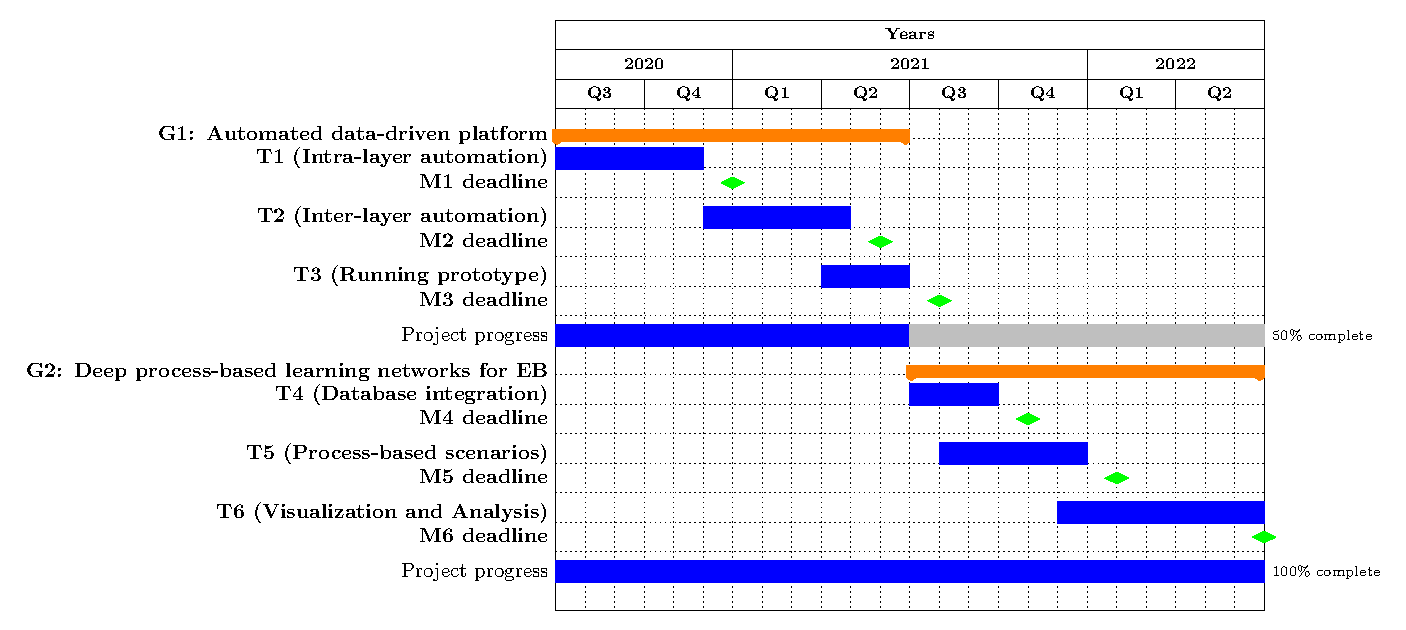
\includegraphics[width=1.1 \textwidth]{FigureMiles.pdf}
\end{center}
\caption{{\small {\bf Figure 5: Work plan and calendar.} The project
    contains two goals ({\bf G1} and {\bf G2}), six tasks and six
    milestones, represented as {\bf T} and {\bf M}, respectively.}}

     \vspace{0.2 in}
     


     \newpage
     \section{Results dissemination and utilization plan}

     {\bf economic and social importance} Significance of the project
     for data science The project will help to improve multilayer
     inference from broad classes of multidimensional data. It will
     bring a class of deep learning networks, deep process-based
     learning networks, to facilitate merging biodiversity research
     and data science. Future versions of the improved automated
     research platform produced during this project will serve as a
     fundamental and applied tool to unfold the processes underlying
     the complex patterns of interdependence among biological, social,
     technological and economical systems.
    
     \newpage
     \section{Budget}
     
     Human resources.
     We require a two-year post-doc: 38648.95 € x 2= 77297.90
     Travel: one-week visit every six months (VME + + postdoc to EAWAG; CJM to IFISC) 300 € transport + 120*5 accommodation + 40 €*5 food= 1300 € x 6 = 7800 €
     one-month stay per semester (postdoc) = 2600 €
     Computation resources: 
     
     Pre-doc 26775,15

     \newpage

\section{References}
\bibliographystyle{unsrtnat}
\bibliography{ref.bib}
\end{document}
